\section{Schachkommentator}

\subsection{Encoder-Decoder Modell}

% ================================================================================ %
\begin{frame}{Encoder-Decoder Modell}
\begin{itemize}
	\item Schachkommentator nimmt Informationen und übersetzt sie in Kommentare
	\item Bereich: Sequence-to-sequence processing
	\begin{itemize}
		\item Abbildung einer Eingabe auf eine Ausgabe
	\end{itemize}
	\item Architektur: Encoder-Decoder Model
	\begin{itemize}
		\item Basierend auf bidirektionalen Long Short-Term Memory (LSTM)
	\end{itemize}
\end{itemize}
\end{frame}




\begin{frame}{Encoder-Decoder Modell}
\begin{itemize}
	\item LSTMs sind eine spezielle Art von Rekurrenten Neuronalen Netzwerken
	\item RNNs sind Neuronale Netzwerke zur Verarbeitung von Datenfolgen
	\begin{itemize}
		\item Outputs werden mit neuen Inputs an das Netzwerk gegeben
		\item Zustand des Netzes repräsentiert Neuronen zu einem bestimmten Zeitpunkt
		\item Netzwerk kann sich an laufende Muster erinnern und auf diese reagieren
	\end{itemize}
	\item Bidirektionale RNNs (Bi-RNN) sind eine Erweiterung von RNNs
	\begin{itemize}
		\item Berücksichtigen sowohl die vorherigen als auch die nachfolgenden Eingabedaten
	\end{itemize}
	\item LSTMs sind spezielle Neuronen
	\begin{itemize}
		\item Bei langen Sequenzen werden die Informationen aus der Vergangenheit nicht korrekt berücksichtigt
		\item LSTMs lösen das Problem
	\end{itemize}
\end{itemize}
\end{frame}




\begin{frame}{Encoder-Decoder Modell}
\begin{itemize}
	\item Encoder-Decoder Modell benutzt Bi-LSTMs
	\begin{itemize}
		\item in der maschinellen Übersetzung verwendet
	\end{itemize}
	\item Besteht aus zwei Teilen: Encoder, Decoder
	\begin{itemize}
		\item Encoder erhält Eingabe von Engine und wandelt diese in andere Darstellung um
		\item Decoder verwendet diese Darstellung und erstellt entsprechende Kommentare
	\end{itemize}
	\item Aufmerksamkeitsmechanismus wird verwendet, um auf wichtige Teile der Sequenz zu konzentrieren
\end{itemize}
\end{frame}




\begin{frame}{Encoder-Decoder Modell}
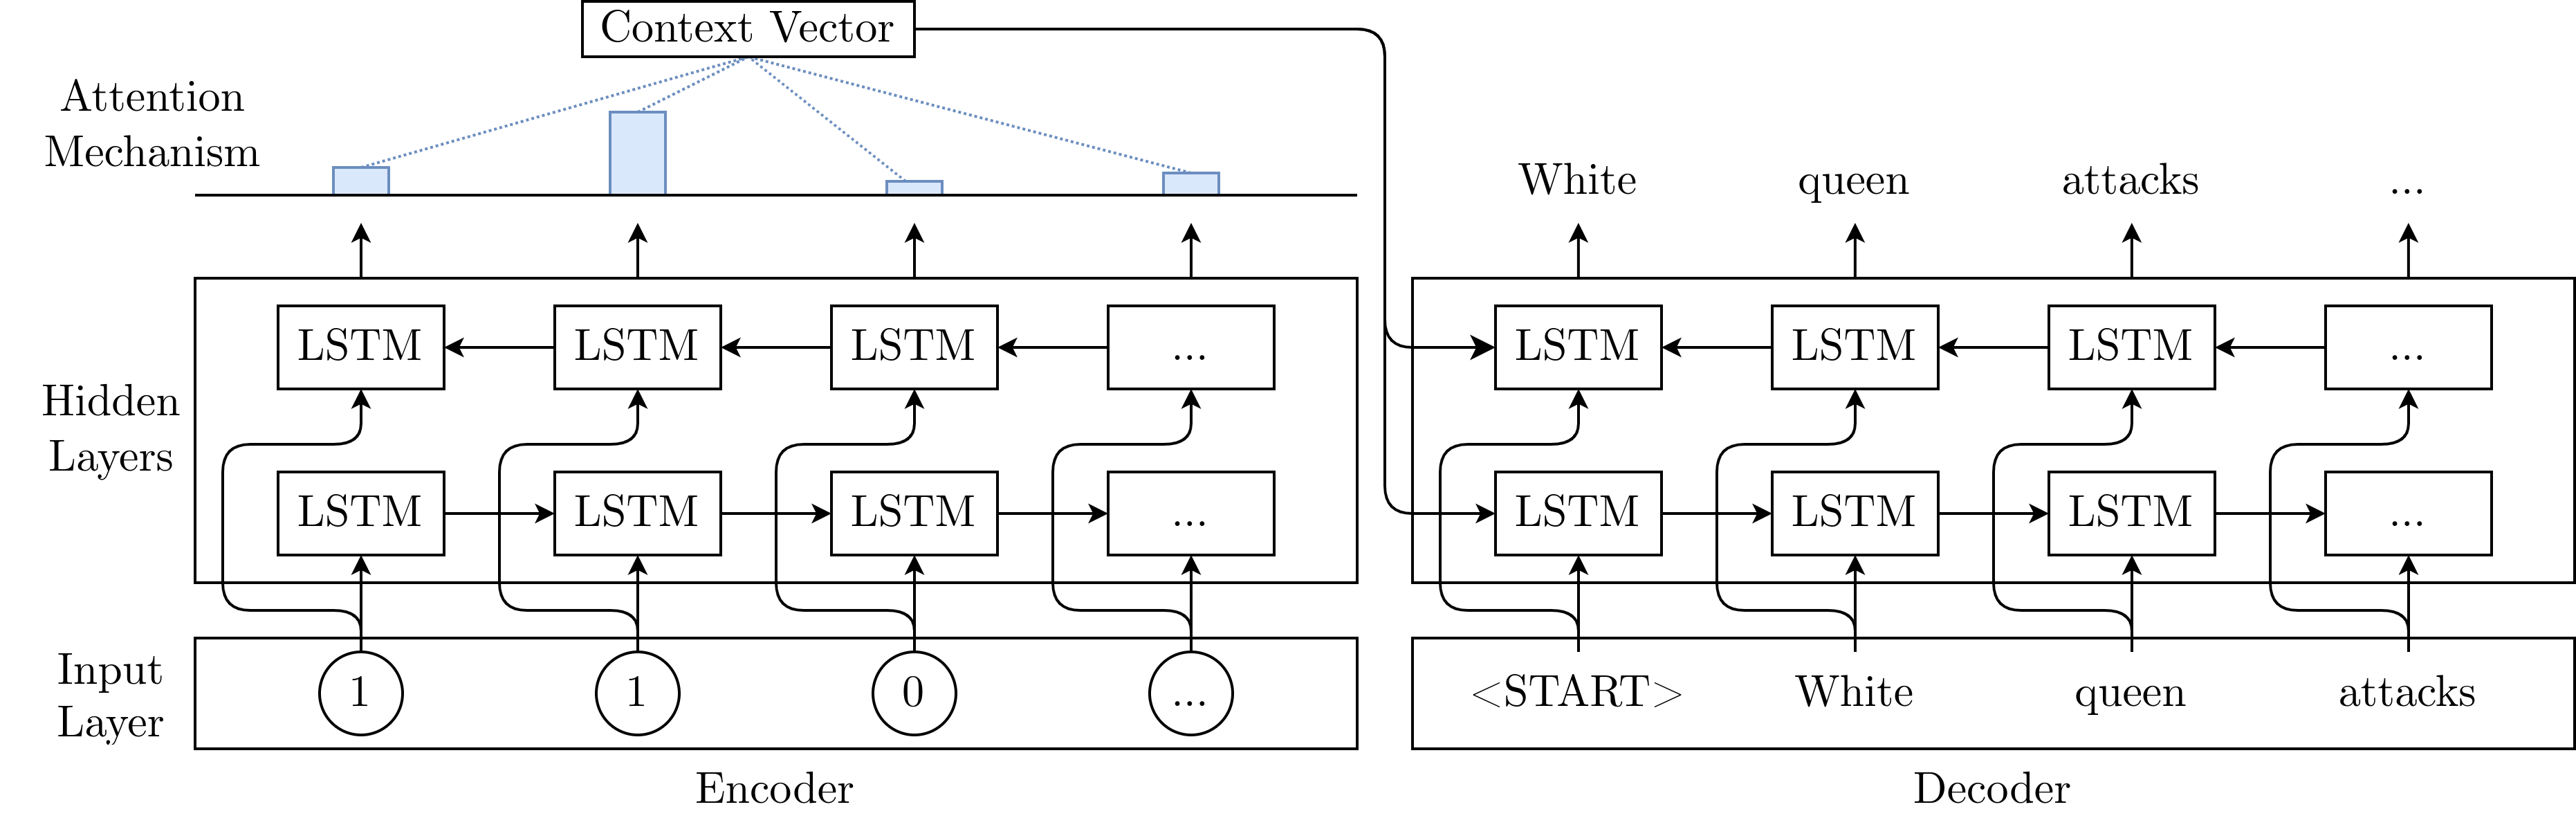
\includegraphics[width=1\textwidth]{graphics/commentator_example/general_approach.png}
\end{frame}
% ================================================================================ %

\subsection{Generationsmodelle}

% ================================================================================ %
\begin{frame}{Generationsmodelle}
\begin{itemize}
	\item Es muss definiert werden, welche Kategorien von Kommentaren generiert werden sollen
	\begin{itemize}
		\item Beschreibung
		\item Qualität
		\item Vergleich
		\item Planung
		\item Kontext
	\end{itemize}
\end{itemize}
\begin{figure}
\centering
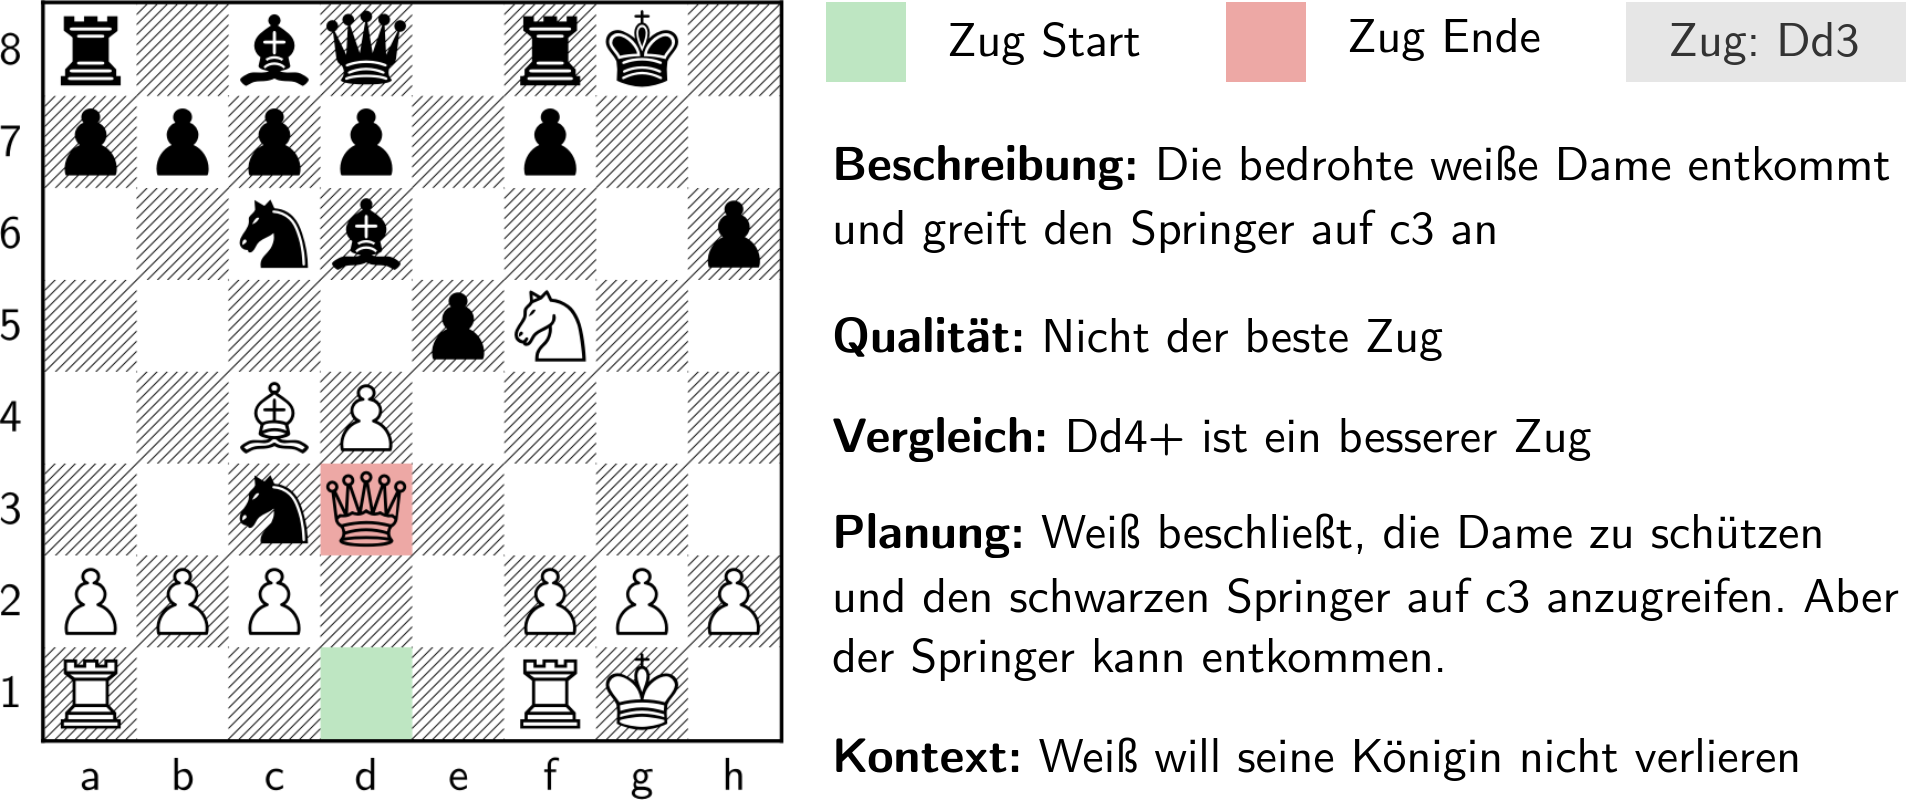
\includegraphics[width=0.55\textwidth]{graphics/commentator_example/commentator.png}
\end{figure}
\end{frame}




\begin{frame}{Generationsmodelle}
\begin{itemize}
	\item Einzelner Kommentator nicht aus
	\item Für jede Kategorie ein Kommentator in Form von Encoder-Decoder Modell (sog. Generationsmodelle)
	\item Generationsmodelle unterscheiden sich im Training
	\begin{itemize}
		\item Unterschiedliche Merkmale und Anzahl an Zügen werden berücksichtigt
	\end{itemize}
\end{itemize}
\end{frame}




\begin{frame}{Generationsmodelle}
\begin{itemize}[<+->]
	\item Zug $m$, Position $b$ 
	\item \textbf{Beschreibung:} $f_{Decoder}(f_{SME}(b_0,m_0)) \rightarrow C_{Beschreibung}$
	\item \textbf{Qualität:} $f_{Decoder}(f_{Encoder}(b_0,b_1,v_1-v_0)) \rightarrow C_{Qualität}$
	\item \textbf{Vergleich:} $f_{Decoder}(f_{MME}(b_1,m_0,b_2,m_1)) \rightarrow C_{Vergleich}$
	\item \textbf{Planung:} $f_{\text{Decoder}}(f_{\text{MME}}((b_2,m_1),(b_3,m_2),(b_4,m_3),...)) \rightarrow C_{\text{Planung}}$
	\item \textbf{Kontext:} $f_{\text{Decoder}}(f_{\text{MME}}((b_1,m_0),(b_2,m_1),(b_3,m_2),(b_4,m_3),...)) \rightarrow C_{\text{Kontext}}$
\end{itemize}
\end{frame}
% ================================================================================ %